%% LyX 2.0.2 created this file.  For more info, see http://www.lyx.org/.
%% Do not edit unless you really know what you are doing.
\documentclass[english]{article}
\usepackage[OT1]{fontenc}
\usepackage[latin9]{inputenc}
\usepackage{geometry}
\geometry{verbose,tmargin=2.5cm,bmargin=2.5cm,lmargin=2.5cm,rmargin=2.5cm}
\usepackage{float}
\usepackage{graphicx}
\usepackage{babel}
\usepackage{lipsum}

\usepackage{tikz}
\usepackage{adjustbox}
\usepackage{pgfplots}
\usepackage{circuitikz}
\usepackage{wrapfig}
\usetikzlibrary{arrows, positioning, calc,shapes}

\usepackage{tikz,amsmath, amssymb,bm,color}
\usetikzlibrary{circuits.logic.US,circuits.logic.IEC,fit}

\newcommand{\mypicture}[1][]{% 1 optional parameter for options for the tikz picture
\begin{tikzpicture}[#1]
\node[draw, circle, fill=yellow!30, inner sep=2mm] (a) {A};
\end{tikzpicture}
}
\newcommand\addvmargin[1]{
  \node[fit=(current bounding box),inner ysep=#1,inner xsep=0]{};
}
\begin{document}

\title{Design of digital integrated systems: optimization of a 16 bit Brent-Kung
adder}


\author{Arnout Devos}

\maketitle

\section{Schematic and optimisation}%\footnotemark[1]}


\subsection{Optimisation}
When trying to minimize the critical delay, first one needs to look at the critical path. The signal on this path needs to travel through a lot of gates (which also drive other gates) which is the determining factor of timing of the adder. Therefore this critical path is the main focus of the timing optimization\footnotemark[1].

When meeting the delay requirements, energy can be optimized. This can be done by decreasing the supply voltage or appropriate sizing of the transistors. In fact upsizing can yield a total reduction in energy (dynamic switching energy) when lowering the supply voltage, taking into account the delay specification.
\footnotetext[1]{\label{note1}Only the critical path going from $a_0b_0$ to $s_{15}$ is optimized keeping the GenerateOverview.m script in mind. The optimization for minimal energy, given all sum outputs are below 650ps delay, is not considered here. In this implementation only the provided transistors are used, so no low-$V_{T}$  or other technologies.}
\subsection{Achitectural optimization}
\begin{itemize}
\item Gate level
\begin{itemize}
\item Moving towards inverted inner stages to remove most inverters. Add inverters where needed to make result correct. An XNOR gate is added to generate $\overline{prop_i}$ in the GenProp block.\\


    \begin{tabular}{ | l | l | l |}
    \hline
\begin{circuitikz}
    \node [draw,circle,fill=orange](klingel) at (8,2.5){};
	\draw (klingel) to[open] ++(0.8,0) node {$=$};
	\addvmargin{0.1cm}
\end{circuitikz} DotoperatorUpper 
&
\begin{circuitikz}
    \node [draw,circle,fill=black!30!orange](klingel) at (8,2.5){};
	\draw (klingel) to[open] ++(0.8,0) node {$=$};
	\addvmargin{0.1cm}
\end{circuitikz} DotoperatorUpperInv
&
GenProp
\\ \hline
\begin{circuitikz}[scale=0.8, transform shape]
	
	\node [nor port] (klingelNOR) at (15,3.7){};
	\node [nand port] (klingelNAND2) at (13,1.5){};
	\node [and port] (klingelAND1) at (13,3) {};
	
	\draw (klingelAND1.in 1) -- ++(-1,0) node[left]{$g_{low}$};
	\draw (klingelAND1.in 2)--++(-0.5,0)node(phigh){}--++(-0.5,0)node[left, color=black]{$p_{high}$};
	\draw (phigh.center) |- (klingelNAND2.in 1);
	\draw (klingelNAND2.in 2) -- ++(-1,0) node[left]{$p_{low}$};	
	\draw (klingelNOR.in 1) -- ++(-3,0) node[left, color=black]{$g_{high}$};
	\draw (klingelNOR.in 2) -- (klingelAND1.out);
	\node [right] at (klingelNOR.out){$\overline{g_{both}}$};
	\node [right] at (klingelNAND2.out){$\overline{p_{both}}$};
	\addvmargin{0.5cm}
\end{circuitikz}
& 
\begin{circuitikz}[scale=0.8, transform shape]
	
	\node [nand port] (klingelNOR) at (15,3.7){};
	\node [nor port] (klingelNAND2) at (13,1.5){};
	\node [or port] (klingelAND1) at (13,3) {};
	
	\draw (klingelAND1.in 1) -- ++(-1,0) node[left]{$\overline{g_{low}}$};
	\draw (klingelAND1.in 2)--++(-0.5,0)node(phigh){}--++(-0.5,0)node[left]{$\overline{p_{high}}$};
	\draw (phigh.center) |- (klingelNAND2.in 1);
	\draw (klingelNAND2.in 2) -- ++(-1,0) node[left]{$\overline{p_{low}}$};	
	\draw (klingelNOR.in 1) -- ++(-3,0) node[left]{$\overline{g_{high}}$};
	\draw (klingelNOR.in 2) -- (klingelAND1.out);
	\node [right] at (klingelNOR.out){$g_{both}$};
	\node [right] at (klingelNAND2.out){$p_{both}$};
	\addvmargin{0.5cm}
\end{circuitikz}
&
\begin{circuitikz}[scale=0.8, transform shape]
    \node [nand port] (genAND) at (5,3){};
	\node [xnor port] (propXOR) at (5,1.5){};

	\node [right] (gen) at (genAND.out){$\overline{gen_i}$};
	\node [right] (prop) at (propXOR.out){$\overline{prop_i}$};
	\draw (genAND.in 1) -- ++(-0.4,0) node (gen1){} -- ++(-0.6,0) node[left]{$a_i$};
	\draw (genAND.in 2) -- ++(-0.5,0) node (gen2){} -- ++(-0.5,0) node[left]{$b_i$};
	\draw (gen1.center) |- (propXOR.in 1);	
	\draw (gen2.center) |- (propXOR.in 2);
	\addvmargin{0.5cm}
\end{circuitikz} 
\\ \hline
    \end{tabular}
\item Remove propagate signals (inverted and non-inverted) from lower dotoperators since only $g_i$ is needed to compute sum.\\
    \begin{tabular}{ | l | l |}
    \hline
\begin{circuitikz}
	\node [draw,circle,fill=green](klingel) at (8,2.5){};
	\draw (klingel) to[open] ++(0.8,0) node {$=$};
\end{circuitikz} DotOperatorLower& \begin{circuitikz}
	\node [draw,circle,fill=black!60!green](klingel) at (0,0){};
	\draw (klingel) to[open] ++(0.8,0) node {$=$};
\end{circuitikz}DotOperatorLowerInv\\ \hline
\begin{circuitikz}[scale=0.8, transform shape]	
		\node [nor port] (klingelNOR) at (15,3.7){};
	%\node [nand port] (klingelNAND2) at (13,1.5){};
	\node [and port] (klingelAND1) at (13,3) {};
	
	\draw (klingelAND1.in 1) -- ++(-1,0) node[left]{$g_{low}$};
	\draw (klingelAND1.in 2)--++(-0.5,0)node(phigh){}--++(-0.5,0)node[left, color=black]{$p_{high}$};
	%\draw (phigh.center) |- (klingelNAND2.in 1);
	%\draw (klingelNAND2.in 2) -- ++(-1,0) node[left]{$p_{low}$};	
	\draw (klingelNOR.in 1) -- ++(-3,0) node[left, color=black]{$g_{high}$};
	\draw (klingelNOR.in 2) -- (klingelAND1.out);
	\node [right] at (klingelNOR.out){$\overline{g_{both}}$};
	%\node [right] at (klingelNAND2.out){$\overline{p_{both}}$};
	\addvmargin{0.5cm}
\end{circuitikz}
&
\begin{circuitikz}[scale=0.8, transform shape]
	%\node [draw,circle](klingel) at (8,2.5){};
	%\draw (klingel) to[open] ++(0.8,0) node {$=$};
	
	\node [nand port] (klingelNOR) at (15,3.7){};
	%\node [nand port] (klingelNAND2) at (13,1.5){};
	\node [or port] (klingelAND1) at (13,3) {};
	
	\draw (klingelAND1.in 1) -- ++(-1,0) node[left]{$\overline{g_{low}}$};
	\draw (klingelAND1.in 2)--++(-0.5,0)node(phigh){}--++(-0.5,0)node[left]{$\overline{p_{high}}$};
	%\draw (phigh.center) |- (klingelNAND2.in 1);
	%\draw (klingelNAND2.in 2) -- ++(-1,0) node[left]{$\overline{p_{low}}$};	
	\draw (klingelNOR.in 1) -- ++(-3,0) node[left]{$\overline{g_{high}}$};
	\draw (klingelNOR.in 2) -- (klingelAND1.out);
	\node [right] at (klingelNOR.out){$g_{both}$};
	%\node [right] at (klingelNAND2.out){$p_{both}$};
	\addvmargin{0.5cm}
\end{circuitikz} \\\hline
    \end{tabular}
\end{itemize}
\newpage
\item Transistor level
\begin{itemize}
\item Attach critical path Generate signal to TOR which is closest to ouptut. Because then, less capacitance has to be charged and signal can therefore propagate faster to the next gate.\\\\
\begin{tabular}{|l|l|}
\hline
\begin{circuitikz}
	\node [draw,circle,fill=green](klingel) at (8,2.5){};
	\draw (klingel) to[open] ++(0.8,0) node {$=$};
\end{circuitikz} DotOperatorLower & \begin{circuitikz}
	\node [draw,circle,fill=black!60!green](klingel) at (0,0){};
	\draw (klingel) to[open] ++(0.8,0) node {$=$};
\end{circuitikz}DotOperatorLowerInv\\ \hline
%\adjustbox{margin={0\width}{0\height} {0\width} {0\height}}{
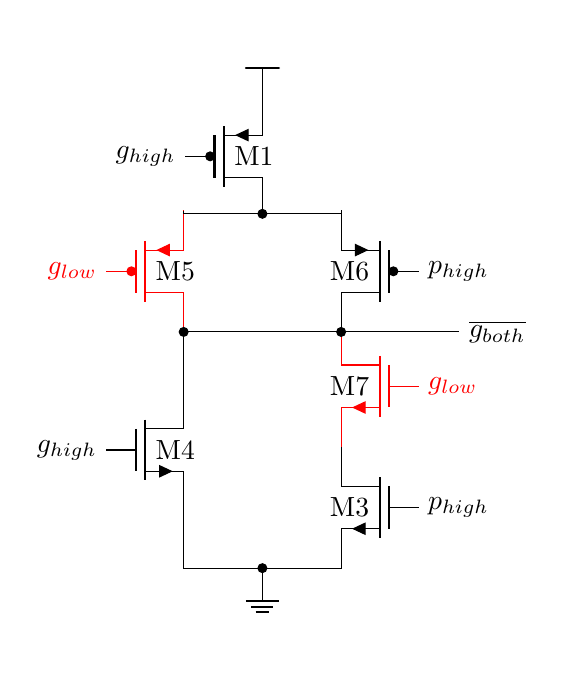
\begin{tikzpicture}
%--------start graphics code --------
%Grid for intial drawing.
%Comment next three lines one typesetting finished
%\def\figHt{5.5};
%\draw[step=0.5,very thin, black!20] (-0.5,-0.5) grid (7,6);
%\foreach \x in {0,...,4} {\node [anchor=north] at (\x,-0.5) {\x};}
%\foreach \y in {0,...,6} {\node [anchor=east] at (-0.5,\y) {\y};}
\ctikzset{tripoles/mos style/arrows}

\coordinate (ground)    at (1,0);
\coordinate (nn1) at ($(ground)+(0,1.5)$);
\coordinate (out) at ($(nn1)+(0,1.5)$);
\coordinate (np1) at ($(out)+(0,1.5)$);
\coordinate (vdd) at ($(np1)+(0,1.5)$);

\draw (ground) node[ground]{};

\draw (ground) ++(1,0) node[nmos,anchor=source,xscale=-1] (M3){};
\draw (M3.base) ++(-0.5,0) node[left]{M3};
\draw (M3.gate) node[right]{$p_{high}$};

\draw (M3.drain) node[nmos,anchor=source,xscale=-1,color=red] (M7){};
\draw (M7.base) ++(-0.5,0) node[left]{M7};
\draw (M7.gate) node[right]{$\color{red}g_{low}$};

\draw (nn1) ++(-1,0) node[nmos] (M4){};
\draw (M4.base) ++(0.5,0) node[right]{M4};
%\draw ($(nn1)+(-1,0)$) -- (M4.drain);
\draw (M4.gate) node[left]{$g_{high}$};
\draw (out) ++(-1,0) node[pmos,anchor=drain,color=red] (M5){};
\draw (M5.base) ++(0.5,0) node[right]{M5};
\draw (M5.gate) node[left]{$\color{red}g_{low}$};
\draw (out) ++(1,0) node[pmos,anchor=drain,xscale=-1] (M6){};
\draw (M6.base) ++(-0.5,0) node[left]{M6};
\draw (M6.gate) node[right]{$p_{high}$};

\draw (vdd) node[pmos,anchor=source] (M1){};
\draw (M1.base) ++(0.5,0) node[right]{M1};
\draw (M1.gate) node[left]{$g_{high}$};

\draw (M5.drain) node[circ]{} to (M6.drain) node[circ]{} -- ++(1.5,0) node[right] {$\overline{g_{both}}$};
\draw (M5.source) |- (np1) node[circ]{} -| (M6.source);
\draw (M4.drain) to (M5.drain);
\draw (M3.source) |- ++(-1,0) node[circ]{} -| (M4.source);

\draw (vdd) node[rground, yscale=-1]{};
\addvmargin{0.5cm}
\end{tikzpicture}
%}
&
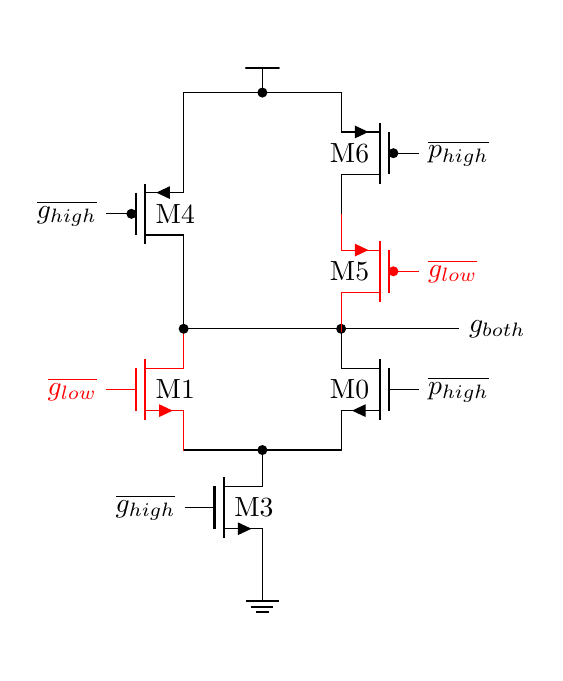
\begin{tikzpicture}

%--------start graphics code --------
%Grid for intial drawing.
%Comment next three lines one typesetting finished
%\def\figHt{5.5};
%\draw[step=0.5,very thin, black!20] (-0.5,-0.5) grid (7,6);
%\foreach \x in {0,...,4} {\node [anchor=north] at (\x,-0.5) {\x};}
%\foreach \y in {0,...,6} {\node [anchor=east] at (-0.5,\y) {\y};}
\ctikzset{tripoles/mos style/arrows}

\coordinate (ground)    at (1,0);
\coordinate (nn1) at ($(ground)+(0,1.5)$);
\coordinate (out) at ($(nn1)+(0,1.5)$);
\coordinate (np1) at ($(out)+(0,1.5)$);
\coordinate (vdd) at ($(np1)+(0,1.5)$);

\draw (ground) node[ground]{};
\draw (nn1) ++(-1,0) node[nmos,anchor=source,color=red] (M1){};
\draw (M1.base) ++(0.5,0) node[right]{M1};
%\draw (ref_node1T) to (Mt1.drain);
\draw (M1.gate) node[left]{$\color{red}\overline{g_{low}}$};
\draw (ground) ++(1,1.5) node[nmos,anchor=source,xscale=-1] (M0){};
\draw (M0.base) ++(-0.5,0) node[left]{M0};
\draw (M0.gate) node[right]{$\overline{p_{high}}$};
\draw (M1.drain) node[circ]{} to (M0.drain) node[circ]{} -- ++(1.5,0) node[right] {$g_{both}$};

\draw (M1.source) |- (nn1) node[circ]{} -| (M0.source);

\draw (ground) node[nmos,anchor=source] (M3){};
\draw (M3.base) ++(0.5,0) node[right]{M3};
\draw (M3.gate) node[left]{$\overline{g_{high}}$};

\draw (np1) ++(-1,0) node[pmos] (M4){};
\draw (M4.base) ++(0.5,0) node[right]{M4};
\draw ($(out)+(-1,0)$) -- (M4.drain);
\draw (M4.gate) node[left]{$\overline{g_{high}}$};
\draw (out) ++(1,0) node[pmos,anchor=drain,xscale=-1,color=red] (M5){};
\draw (M5.base) ++(-0.5,0) node[left]{M5};
\draw (M5.gate) node[right]{$\color{red}\overline{g_{low}}$};
\draw (np1) ++(1,0) node[pmos,anchor=drain,xscale=-1] (M6){};
\draw (M6.gate) node[right]{$\overline{p_{high}}$};
\draw (M6.base) ++(-0.5,0) node[left]{M6};
%\draw (M4.source) |- node[circ]{} (M6.source);
\draw (M6.source) |- ++(-1,0) node[circ]{} -| (M4.source);

\draw (vdd) node[rground, yscale=-1]{};
\addvmargin{0.5cm}
\end{tikzpicture}
\\ \hline
\end{tabular}
%%%%%%%%%%%%%%%%%%%%%%%%%%%%%%%%%%%%%%%%%%%%%%%%%%%%%%%%%%%%%%%%%%%%%%%%%%%%%%%%%%%%%%%%%%%%%%%%%
\\
\item Use passgate logic XOR (genprop and sums) to minimize switching energy. However still use a regular XOR on critical path for speed.
\item Since the critical path starts at the XNOR gate with $prop_{1}$, the wiring to the dotoperator will be done in such a way that $prop_{1}$ is connected to the transistors closest to the output.
\end{itemize}
\item Structural level
\begin{itemize}
\item Use minimal inverters (see section \ref{sec:sizing}) to correct for the optimization of the critical path. This means that certain non-critical paths will need to be converted to their inverted counterpart again, because a minimal inverter has been used to minimally load the critical path.
\end{itemize}
\end{itemize}
\subsection{Sizing} \label{sec:sizing} 
\begin{itemize}
\item Decrease sizing of all transistors loading the critical path to minimal sizing for both pMOS and nMOS to minimize energy consumption.

\begin{itemize}
\item 
\begin{tabular}{p{9cm} p{3cm}}
    \vspace{0pt} 
    In case the critical path is loaded with more than 2 transistors on the non-critical path, minimal inverters are inserted as 'inverting buffers': relative size 1 pMOS \& size 1 nMOS to load the  preceding gate (on the critical path) with as little capacitance as possible.
    & 
    \vspace{0pt}
    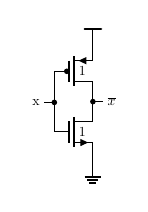
\begin{tikzpicture}[scale=0.5, transform shape]
\ctikzset{tripoles/mos style/arrows}

\coordinate (ground)    at (0,0);
\coordinate (out) at ($(ground)+(0,1.5)$);
\coordinate (vdd) at ($(out)+(0,1.5)$);

\draw (ground) node[ground]{};
\draw (out) node[nmos,anchor=drain] (M1){};
\draw (M1.base) ++(0.5,0) node[right]{1};
\draw (out) node[pmos,anchor=drain] (M2){};
\draw (M2.base) ++(0.5,0) node[right]{1};

\draw (M1.gate) -- ++(0,0.75) node[circ]{} -- (M2.gate);
\draw (M1.gate) ++(0,0.75) -- ($(M1.gate) +(-0.25,0.75)$) node[left]{x};
\draw (M1.drain) node[circ]{} -- ++(0.25,0) node[right] {$\overline{x}$};

\draw (vdd) node[rground, yscale=-1]{};
\end{tikzpicture}\\
\end{tabular}
\end{itemize}
\item Scale sizing on critical path for optimal energy and delay.
\begin{itemize}
\item Since minimal energy is the goal, a more than exponential sizing approach will yield the best results. 
\item Make transistors connecting the critical path transistor to $V_{DD}$ or $ground$ arbitrarily big to provide a very good conducting path in case of a critical change. Remark that the increased capacitance which comes with this increase in width doesn't influence the timing since the intermediate node has already settled to the 'correct' value when the critical signal arrives.
\end{itemize}
\end{itemize}
\subsection{Task}
All in all you should have about two pages of explication (including
the header).
\section{Results}
Please fill in table \ref{table2}. Additional columns may be added, but provide at 
least one column with the data for the point with delay 650 ps.

\begin{table}[b]
\centering
\begin{tabular}{ |l|r| }
\hline
Delay & 650 ps \\
Supply & 0.883 V \\
Switching Energy & 80 fJ \\
DC power & 1.31 nW \\
\hline
\end{tabular}
\caption{Final performance of the circuit}
\label{table2}
\end{table}

%\newpage{}


\subsection{Schematic}

\begin{figure}[H]
\begin{centering}
\includegraphics[angle=90,width=0.9\textwidth]{figures/DelayEnergy_tex}
\par\end{centering}
\caption{Schematic of the optimised adder}
\end{figure}

\iffalse
\begin{table}[b]
\centering
\begin{tabular}{ |c||c| }
\hline
\begin{circuitikz}
\node [draw,circle](klingel) at (8,2.5){};
	\draw (klingel) to[open] ++(0.8,0) node {$=$};
\end{circuitikz} DotoperatorUpper & \begin{circuitikz}
\node [draw,circle](klingel) at (8,2.5){};
	\draw (klingel) to[open] ++(0.8,0) node {$=$};
\end{circuitikz} DotoperatorUpperInv\\ \hline
\begin{circuitikz}
	
	\node [nor port, color=blue] (klingelNOR) at (15,3.7){};
	\node [nand port] (klingelNAND2) at (13,1.5){};
	\node [and port, color=blue] (klingelAND1) at (13,3) {};
	
	\draw[color=blue] (klingelAND1.in 1) -- ++(-1,0) node[left, color=black]{$g_{low}$};
	\draw[color=blue] (klingelAND1.in 2)--++(-0.5,0)node(phigh){}--++(-0.5,0)node[left, color=black]{$p_{high}$};
	\draw (phigh.center) |- (klingelNAND2.in 1);
	\draw (klingelNAND2.in 2) -- ++(-1,0) node[left]{$p_{low}$};	
	\draw[color=blue] (klingelNOR.in 1) -- ++(-3,0) node[left, color=black]{$g_{high}$};
	\draw[color=blue] (klingelNOR.in 2) -- (klingelAND1.out);
	\node [right] at (klingelNOR.out){$\overline{g_{both}}$};
	\node [right] at (klingelNAND2.out){$\overline{p_{both}}$};
\end{circuitikz} & \begin{circuitikz}
	
	\node [nand port] (klingelNOR) at (15,3.7){};
	\node [nor port] (klingelNAND2) at (13,1.5){};
	\node [or port] (klingelAND1) at (13,3) {};
	
	\draw (klingelAND1.in 1) -- ++(-1,0) node[left]{$\overline{g_{low}}$};
	\draw (klingelAND1.in 2)--++(-0.5,0)node(phigh){}--++(-0.5,0)node[left]{$\overline{p_{high}}$};
	\draw (phigh.center) |- (klingelNAND2.in 1);
	\draw (klingelNAND2.in 2) -- ++(-1,0) node[left]{$\overline{p_{low}}$};	
	\draw (klingelNOR.in 1) -- ++(-3,0) node[left]{$\overline{g_{high}}$};
	\draw (klingelNOR.in 2) -- (klingelAND1.out);
	\node [right] at (klingelNOR.out){$g_{both}$};
	\node [right] at (klingelNAND2.out){$p_{both}$};
\end{circuitikz} \\ \hline \hline
\begin{circuitikz}
	\node [draw,circle,fill=green](klingel) at (8,2.5){};
	\draw (klingel) to[open] ++(0.8,0) node {$=$};
\end{circuitikz} DotOperatorLower& \begin{circuitikz}
	\node [draw,circle](klingel) at (0,0){};
	\draw (klingel) to[open] ++(0.8,0) node {$=$};
\end{circuitikz}DotOperatorLowerInv\\ \hline
\begin{circuitikz}	
		\node [nor port, color=green] (klingelNOR) at (15,3.7){};
	%\node [nand port] (klingelNAND2) at (13,1.5){};
	\node [and port, color=green] (klingelAND1) at (13,3) {};
	
	\draw[color=green] (klingelAND1.in 1) -- ++(-1,0) node[left, color=red]{$g_{low}$};
	\draw[color=green] (klingelAND1.in 2)--++(-0.5,0)node(phigh){}--++(-0.5,0)node[left, color=black]{$p_{high}$};
	%\draw (phigh.center) |- (klingelNAND2.in 1);
	%\draw (klingelNAND2.in 2) -- ++(-1,0) node[left]{$p_{low}$};	
	\draw[color=green] (klingelNOR.in 1) -- ++(-3,0) node[left, color=black]{$g_{high}$};
	\draw[color=green] (klingelNOR.in 2) -- (klingelAND1.out);
	\node [right] at (klingelNOR.out){$\overline{g_{both}}$};
	%\node [right] at (klingelNAND2.out){$\overline{p_{both}}$};
\end{circuitikz}
&
\begin{circuitikz}
	%\node [draw,circle](klingel) at (8,2.5){};
	%\draw (klingel) to[open] ++(0.8,0) node {$=$};
	
	\node [nor port] (klingelNOR) at (15,3.7){};
	%\node [nand port] (klingelNAND2) at (13,1.5){};
	\node [and port] (klingelAND1) at (13,3) {};
	
	\draw (klingelAND1.in 1) -- ++(-1,0) node[left]{$\overline{g_{low}}$};
	\draw (klingelAND1.in 2)--++(-0.5,0)node(phigh){}--++(-0.5,0)node[left]{$\overline{p_{high}}$};
	%\draw (phigh.center) |- (klingelNAND2.in 1);
	%\draw (klingelNAND2.in 2) -- ++(-1,0) node[left]{$\overline{p_{low}}$};	
	\draw (klingelNOR.in 1) -- ++(-3,0) node[left]{$\overline{g_{high}}$};
	\draw (klingelNOR.in 2) -- (klingelAND1.out);
	\node [right] at (klingelNOR.out){$g_{both}$};
	%\node [right] at (klingelNAND2.out){$p_{both}$};
\end{circuitikz} \\
\hline
\end{tabular}
\caption{Different DotOperators used in Adder}
\label{table1}
\end{table}
\fi
\end{document}